\documentclass[../Main.tex]{subfiles}

\tikzstyle{startstop} = [
    rectangle,
    rounded corners=1.5em,
    minimum height=1cm,
    minimum width=3cm,
    text width=3cm, 
    text centered, 
    draw=gray!60, 
    fill=gray!20
]

\tikzstyle{process} = [
    rectangle, 
    rounded corners, 
    minimum width=3cm, 
    minimum height=1cm,
    text centered, 
    text width=3cm, 
    draw=gray!60, 
    fill=gray!20
]

\tikzstyle{decision} = [
    diamond, 
    minimum width=4cm, 
    minimum height=0.5cm, 
    text centered, 
    draw=gray!60, 
    fill=gray!20
]

\tikzstyle{arrow} = [thick,->,>=stealth, draw=gray!90]

\begin{document}

The preceding chapters of this document have meticulously delineated the architectural framework and the technological foundations employed in the system's development process. However, without distinct solutions and initiatives, the system might have remained indistinguishable within the extensive landscape of business solutions and unsuitable in other environments like Vietnam. This chapter aims to shed light on how the issues are identified in the development progress of the project and the personalized strategies and innovations that contributed to the system's uniqueness and enhanced its efficacy and relevance in a dynamic business environment.

\section{Display custom text}
In the development process, the system encounters an issue when the user wants to display Vietnamese language texts and other special characters not in the ASCII character map. Vietnamese, with its complex diacritical marks and distinct character set, demands a high degree of precision in rendering, a task that is particularly challenging given the inherent limitations and operational mechanics of e-paper displays. This section will focus on how normal text is stored and processed in constrained environments like ESP32 and the problem of performance over resource usage. 

\subsection{UTF-8 vs. UTF-16}
\label{encoding}
UTF-8 and UTF-16 are both encoding formats used for representing text in computers, each with its unique handling of character sets, including special characters like those in the Vietnamese language. Unlike ASCII, where each character uses one byte to store, UTF-8 uses one to four bytes per character, making it highly capable of 1112064 valid character codes while still being backward-compatible with ASCII's old code. On the other hand, UTF-16 uses fixed-length two or four bytes per character, balancing the space efficiency of UTF-8 and the simplicity of fixed-length encoding. In the scope of this project, both encoding formats are compatible with processing Vietnamese characters to display on screen, each with its unique strengths and weaknesses. UTF-8, while enhancing the efficiency in memory and storage, still has drawbacks when parsing variable-length characters. The ESP32 must decode UTF-8 encoded strings into Unicode code points and then translate these into bitmaps. This process can lead to processing overhead and is more CPU-intensive compared to dealing with a fixed-length encoding like UTF-16.

\subsection{Two ways of process and display text}
\label{2-ways-process}
To be displayed properly on the screen, the text has to be converted to a bitmap image, stored in the form of an array of bytes. This process can be achieved in two ways: converting from an image of characters (Figure \ref{fig:thedotfactory}) or directly from the font file to corresponding byte arrays. The main goal of both two conversion ways is to create a mapping from every character to the corresponding bytes array, which is a step in the display process illustrated in Figure \ref{2-ways-process}. Due to the specific nature of frequently displaying Vietnamese characters, the project uses the second option, with the help of the TheDotFactory tool, to convert all the Vietnamese and Latin characters mapped to the byte arrays.
\begin{figure}[h]
    \centering
    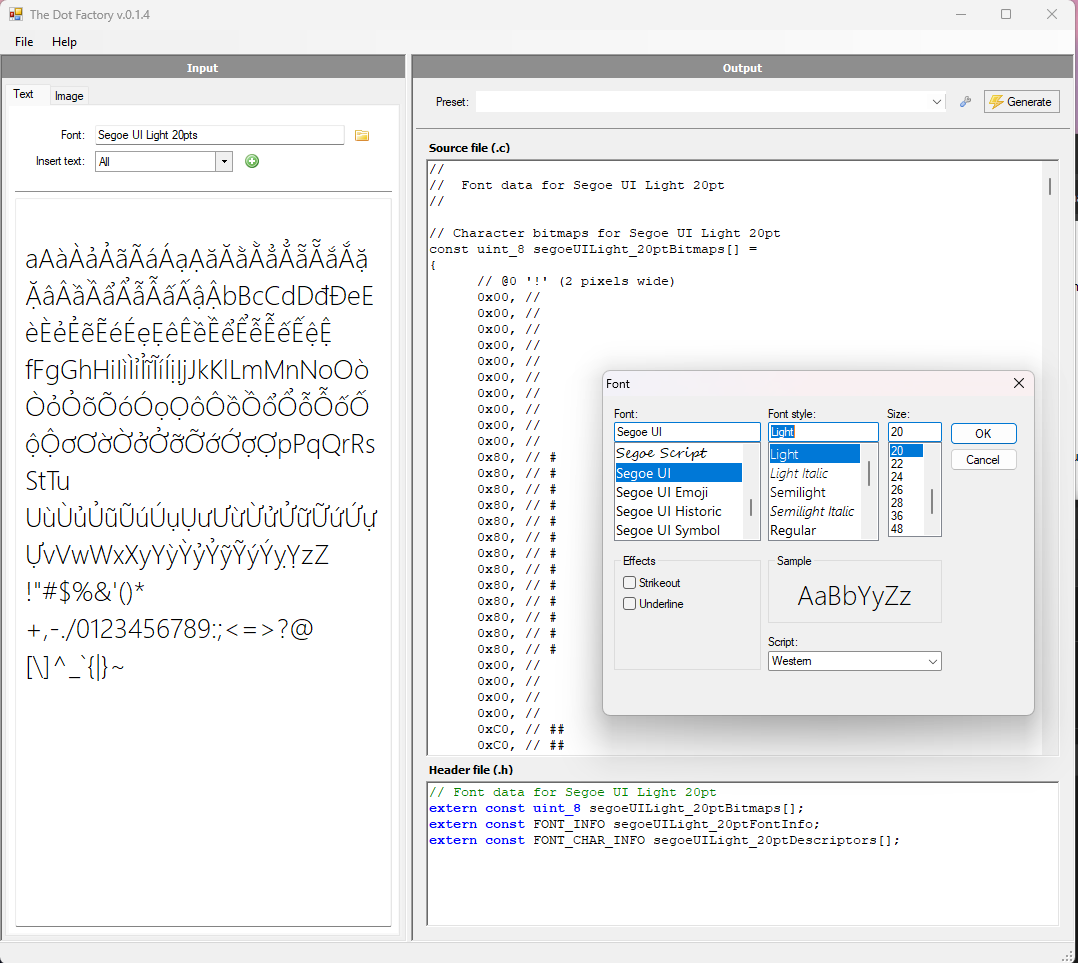
\includegraphics[width=0.8\linewidth]{doc/imgs/thedotfactory.png}
    \caption{UI of TheDotFactory tool}
    \label{fig:thedotfactory}
\end{figure}

\begin{center}
    {\fontsize{10pt}{8pt}\selectfont 
        \begin{tikzpicture}[node distance=2.5cm, auto]
            \node (proc1) [process, minimum width=4cm, text width = 4cm, minimum height = 1.5cm] {\textbf{Iterate over string}\\\verb|“àăảBcd123@”|};
            \node (proc2) [process, below of=proc1, minimum width=4cm, text width = 4cm, minimum height = 1.5cm] {\textbf{Character}\\\verb|'à'|};
            \node (proc3) [process, right of=proc2, minimum width=4cm, text width = 4cm, minimum height = 1.5cm, xshift=3cm] {\textbf{Bytes-array lookup}\\"0x00 0xF2 0x21 ..."};
            \node (proc4) [process, right of=proc1, minimum height = 1.5cm, xshift=3cm] {\textbf{Display}};
            
            \draw [arrow] (proc1) -- (proc2);
            \draw [arrow] (proc2) -- (proc3);
            \draw [arrow] (proc3) -- (proc4);
            \draw [arrow] (proc4) -- (proc1);
        \end{tikzpicture}
    }
\end{center}

In the text-processing task, looking for the bytes array of each character is the most resource-consuming task, especially in an extensive character set. In resource-limited systems like ESP32-c3supermini in the project, it is crucial to balance between saving as many resources as possible and processing data in a reasonable time. However, the way data is organized in the exported file from TheDotFactory does not effectively solve the problem of processing performance and resource conservation when having to store and process 228 different characters, including Latin letters, accented Vietnamese, special characters, and numbers. This issue, combined with the encoding formats discussed above, leads to two ways of storing and mapping from the character to its corresponding bytes array, with a big difference in performance and resource usage between the two.

\subsection{First Solution}
The first of the two solutions mentioned above is a practical and straightforward approach focusing on the flexibility and scalability of the character set. The mapped character set is stored in an array of multiple character map definitions, where each character is associated with a structure that contains its display properties (width) and the corresponding byte array for rendering (code structure below), making the retrieval of byte data for each character straightforward and intuitive. This method is particularly suited for systems where a direct and easy way to access the display data for each character is highly recommended, especially for a fixed and known set of characters.

{\fontsize{8pt}{8pt}\selectfont 
    \begin{verbatim}
  typedef struct 
  {
    char16_t * chr;                                     // index character, utf-16
    uint8_t width;                                      // dynamic width
    const char matrix[MAX_HEIGHT_FONT*MAX_WIDTH_FONT/8];// bytes-array (41*32/8)
  } FT_IDX;
  
  typedef struct
  {    
    const FT_IDX *table;
    uint16_t size;
    uint8_t Height;
  } cFONT;   // custom Font
    \end{verbatim}
}
The index character \verb|chr| defined in the struct above uses UTF-16 as the encoding format. Although it is not as memory-efficient as UTF-8 encoding format as discussed in section \ref{encoding}, UTF-16 encoding brings ease of character comparisons while UTF-8 requires checking multiple bytes for non-ASCII characters (above 126), which appear the most frequently in the Vietnamese language. The flow chart below shows the details of the process displaying a Vietnamese string on the screen.
\begin{center}
    {\fontsize{9pt}{8pt}\selectfont 
        \begin{tikzpicture}[node distance=2.5cm, auto]
            \node (start) [startstop, minimum width=4cm, minimum height = 1.5cm, rounded corners=2.4em] {\textbf{UTF-8 String} \verb|“àăảBcd123@”|};
            \node (proc1) [process, below of=start, minimum width=4cm, text width = 4cm, minimum height = 1.5cm] {\textbf{Convert to UTF-16}\\\verb|u“àăảBcd123@”|};
            \node (proc2) [process, below of=proc1, minimum width=4cm, text width = 4cm, minimum height = 1.5cm] {\textbf{Iterate over string}\\\verb|u'à'|};
            \node (dec1) [decision, below of=proc2] {\textbf{End of string?}};
            \node (stop) [startstop, right of=dec1, xshift=2cm] {\textbf{Finish}};
            \node (proc3) [process, below of=dec1, minimum width=4cm, text width = 4cm] {\textbf{Search in character map}};
            \node (dec2) [decision, below of=proc3, text width = 1.8cm] {\textbf{Found index character?}};
            \node (proc4) [process, right of=dec2, xshift=2cm] {\textbf{Get bytes-array}};
            \node (proc5) [process, below of=proc4] {\textbf{Display}};
            
            \draw [arrow] (start) -- (proc1);
            \draw [arrow] (proc1) -- (proc2);
            \draw [arrow] (proc2) -- (dec1);
            \draw [arrow] (dec1) -- node[anchor=south] {Yes} (stop);
            \draw [arrow] (dec1) -- node[anchor=east] {No} (proc3);
            \draw [arrow] (proc3) -- (dec2);
            \draw [arrow] (dec2) -- node[anchor=south] {Yes} (proc4);
            \draw [arrow] (dec2.west) -- ++(-0.5,0) -- node[midway, left] {No} ++(0,2.5) -- (proc3.west);
            \draw [arrow] (proc4) -- (proc5);
            \draw [arrow] (proc5.west) -- ++(-6.2,0) -- ++(0,10) -- (proc2.west);
        \end{tikzpicture}
    }
\end{center}

In terms of memory, this method stores a character set and occupies around 169 bytes per character map for 228 characters. For all 228 characters in the set, this method occupies a total of \(169 \times 228 = 38,532\) bytes or 37 kilobytes. This is also affected by the compiler padding and alignment, so this calculation provides an approximated number based on the struct layout of the character set. However, most bytes-arrays of each character in this project only take up around 40 bytes on average, which, in fact, only costs \(228 \times 40 = 9,120\) bytes, or 9 kilobytes of actual data, meaning there are still many redundant space unusable with this method. Also, the data of the processing task, which includes the converted UTF-16 string and other variables in the process, is not accounted for, making an even higher total memory occupation. Currently, this is not a big problem with ESP32-c3supermini, but when the system gets more complicated or is implemented in smaller microcontrollers, another approach is highly recommended to balance performance and resources.

\subsection{Second Solution}
The second solution uses the segment method combined with the lookup table, optimizing resource and time efficiency even more, especially in a constrained environment. In this method, each character is not directly mapped to its bytes-array but to the start index and the length of its array, and the array containing these character maps is a lookup table. In this way, the bytes array will be stored in one extensive single array, which reduces memory overhead significantly compared to the first straightforward method. Also, having a map that links each character to its corresponding byte range in the array allows for fast lookup and retrieval, making the rendering process more efficient, especially when dealing with larger sets of characters or more frequent character lookups, as would be the case when rendering text from strings.

However, finding the index character in the lookup table is also a time- and resource-consuming task as it usually iterates through the array to get the data corresponding to the character. Therefore, the lookup table is divided into three segments based on the use frequency, and each segment contains a group of characters that share mostly the same frequency range. This will boost the lookup time as it does not require iterating over a single array to find needed information. However, because Vietnamese characters in the UTF-8 table are distributed differently from the use frequency and the limited time of the project, the segments are still divided based on the UTF-8 table, with the first segment containing characters of ASCII table, the second segment containing the first half of Vietnamese character set, and the third segment containing the second half. To speed up the lookup process in each segment, the index character is converted to the corresponding Unicode point, and binary search is also used, which is implemented in \verb|binarySearchInSegment()| function in the code structure shown below.

{\fontsize{8pt}{8pt}\selectfont 
    \begin{verbatim}
  typedef struct 
  {
    int chr; // index character, Unicode point
    uint8_t width;  // dynamic width, used to determine the byte array's length
    int index;  // start index at byte map table
  } FT_MAP;

  typedef struct
  {    
    const FT_MAP *ASCII_table; // segmentSize = 95 characters from 32 to 126
    const FT_MAP *vn_table;    // segmentSize = 
    const FT_MAP *VN_table;    // segmentSize = 
    uint8_t Height;            //character's height, in pixels
  
    const FT_MAP * binarySearchInSegment(
      int unicodePoint, 
      const FT_MAP* segment, 
      size_t segmentSize
    );
    
    const char *table;
  } cFONT_SEGMENT;   // custom Font with Segment Management
    \end{verbatim}
}

 The flow chart below shows the details of the process displaying a Vietnamese string on the screen in the second method.

\begin{center}
    {\fontsize{7pt}{8pt}\selectfont 
        \begin{tikzpicture}[node distance=2cm, auto]
            \node (start) [startstop, minimum width=3cm, minimum height = 1.2cm, rounded corners=2.5em] {\textbf{UTF-8 String} \verb|“àăảBcd123@”|};
            \node (proc1) [process, below of=start, minimum width=1cm, text width = 4cm, minimum height = 1cm, yshift=0.5cm] {\textbf{Iterate over string}\\\verb|“à”|};
            \node (dec1) [decision, below of=proc1] {\textbf{End of string?}};
            \node (proc2) [process, below of=dec1, minimum width=2cm, text width = 4cm, minimum height = 1cm, yshift=-0.2cm] {\textbf{Convert to Unicode point}\\\verb|224|};
            \node (stop) [startstop, right of=proc2, xshift=2cm, rounded corners=2em] {\textbf{Finish}};
            \node (dec2) [decision, below of=proc2, text width = 2cm, minimum width=3cm, minimum height=1cm, yshift=-0.4cm] {\textbf{Compare to segment ranges}};
            \node (proc3) [process, below of=dec2, minimum width=4cm, text width = 7cm, minimum height = 2cm, yshift=-1.3cm] {\textbf{Binary search in corresponding segment}\\(Segment 1: Latin characters)\\(Segment 2: First-half Vietnamese characters)\\(Segment 3: Second-half Vietnamese characters)};
            \node (dec3) [decision, below of=proc3, text width = 1.8cm, yshift=-1cm] {\textbf{Found index character?}};
            \node (proc4) [process, below of=dec3, yshift=-0.6cm] {\textbf{Get bytes-array from bytes table}};
            \node (proc5) [process, below of=proc4] {\textbf{Display}};
            
            \draw [arrow] (start) -- (proc1);
            \draw [arrow] (proc1) -- (dec1);
            \draw [arrow] (dec1.east) -- node[anchor=south] {Yes} ++(2,0) -- (stop.north);
            \draw [arrow] (dec1) -- node[anchor=east] {No} (proc2);
            \draw [arrow] (proc2) -- (dec2);
            \draw [arrow] (dec2) -- node[anchor=east] {Found} (proc3);
            \draw [arrow] (dec2.east) -- node[anchor=south] {Not found} ++(2.5,0) -- (stop.south);
            \draw [arrow] (proc3) -- (dec3);
            \draw [arrow] (dec3.east) -- node[anchor=south] {Not found} ++(2.5,0)  -- ++(0,3) -- (proc3.east);
            \draw [arrow] (dec3) -- node[anchor=east] {Found} (proc4);
            \draw [arrow] (proc4) -- (proc5);
            \draw [arrow] (proc5.west) -- ++(-3,0) -- ++(0,17.5) -- (proc1.west);
        \end{tikzpicture}
    }
\end{center}

In this solution, Unicode Point is used instead of the original UTF-8 encoding format, which performs better in character comparisons than UTF-8 and UTF-16. However, a function to convert from UTF-8 characters to Unicode points is still needed, and the lookup array in each segment is sorted in ascending order based on the Unicode points of its character elements for the binary search function. In terms of memory, each character map takes up around only 9 bytes, and the single bytes array occupies around 9000 bytes on average, making a total of \(9\times228+9000=11,052\) bytes, or 11 kilobytes, of the character set. Also, this calculation is estimated on the code structure, not taking the data during the process into account, and actual memory usage might slightly differ due to factors like alignment and padding specific to the compiler and the architecture.

About performance, ...

Overall, the logic for accessing and using the data in this second solution becomes slightly more complex, requiring correctly handling the mapping and indexing into the byte array. However, this method leverages the advantages of both segmentation and binary search, effectively reducing the search space and improving lookup times, making it well-suited for handling a large set of characters efficiently on systems with limited resources like the ESP32.

\section{Shapes and Bitmap Images}
\section{Partial Display}
a
\section{ESP32 Optimization}
\subsection{Battery}
\subsection{Serial Port}

\section{RabbitMQ}

\section{Security and vulnerabilities}
A secure and reliable connection is mandatory in a system that includes many devices communicating with each other and storing sensitive data. This project, however, had to go through a system hack that resulted in all users' data being deleted and sold on the black market. This experience, together with other security issues in the development process, has brought an urgency to enhance the system's security.
\subsection{MongoDB Hack}
Currently, MongoDB in the system is configured securely with the user's credentials and is being proxied behind a secure connection. However, on the first days of the development, with rudimentary configurations and exposing many vulnerabilities, the MongoDB server is "open" to the public with little protection from the system firewall. Several hacks targeting the MongoDB databases via the open port 27017 of the MongoDB server have been conducted by a hacker who deleted all collections and overwrote them with a recovery message. This message demanded a payment of 0.025 BTC (equivalent to \$1,000) to recover the data; otherwise, the data will be "published on the darknet forums on the TOR network".
\begin{figure}[H]
    \centering
    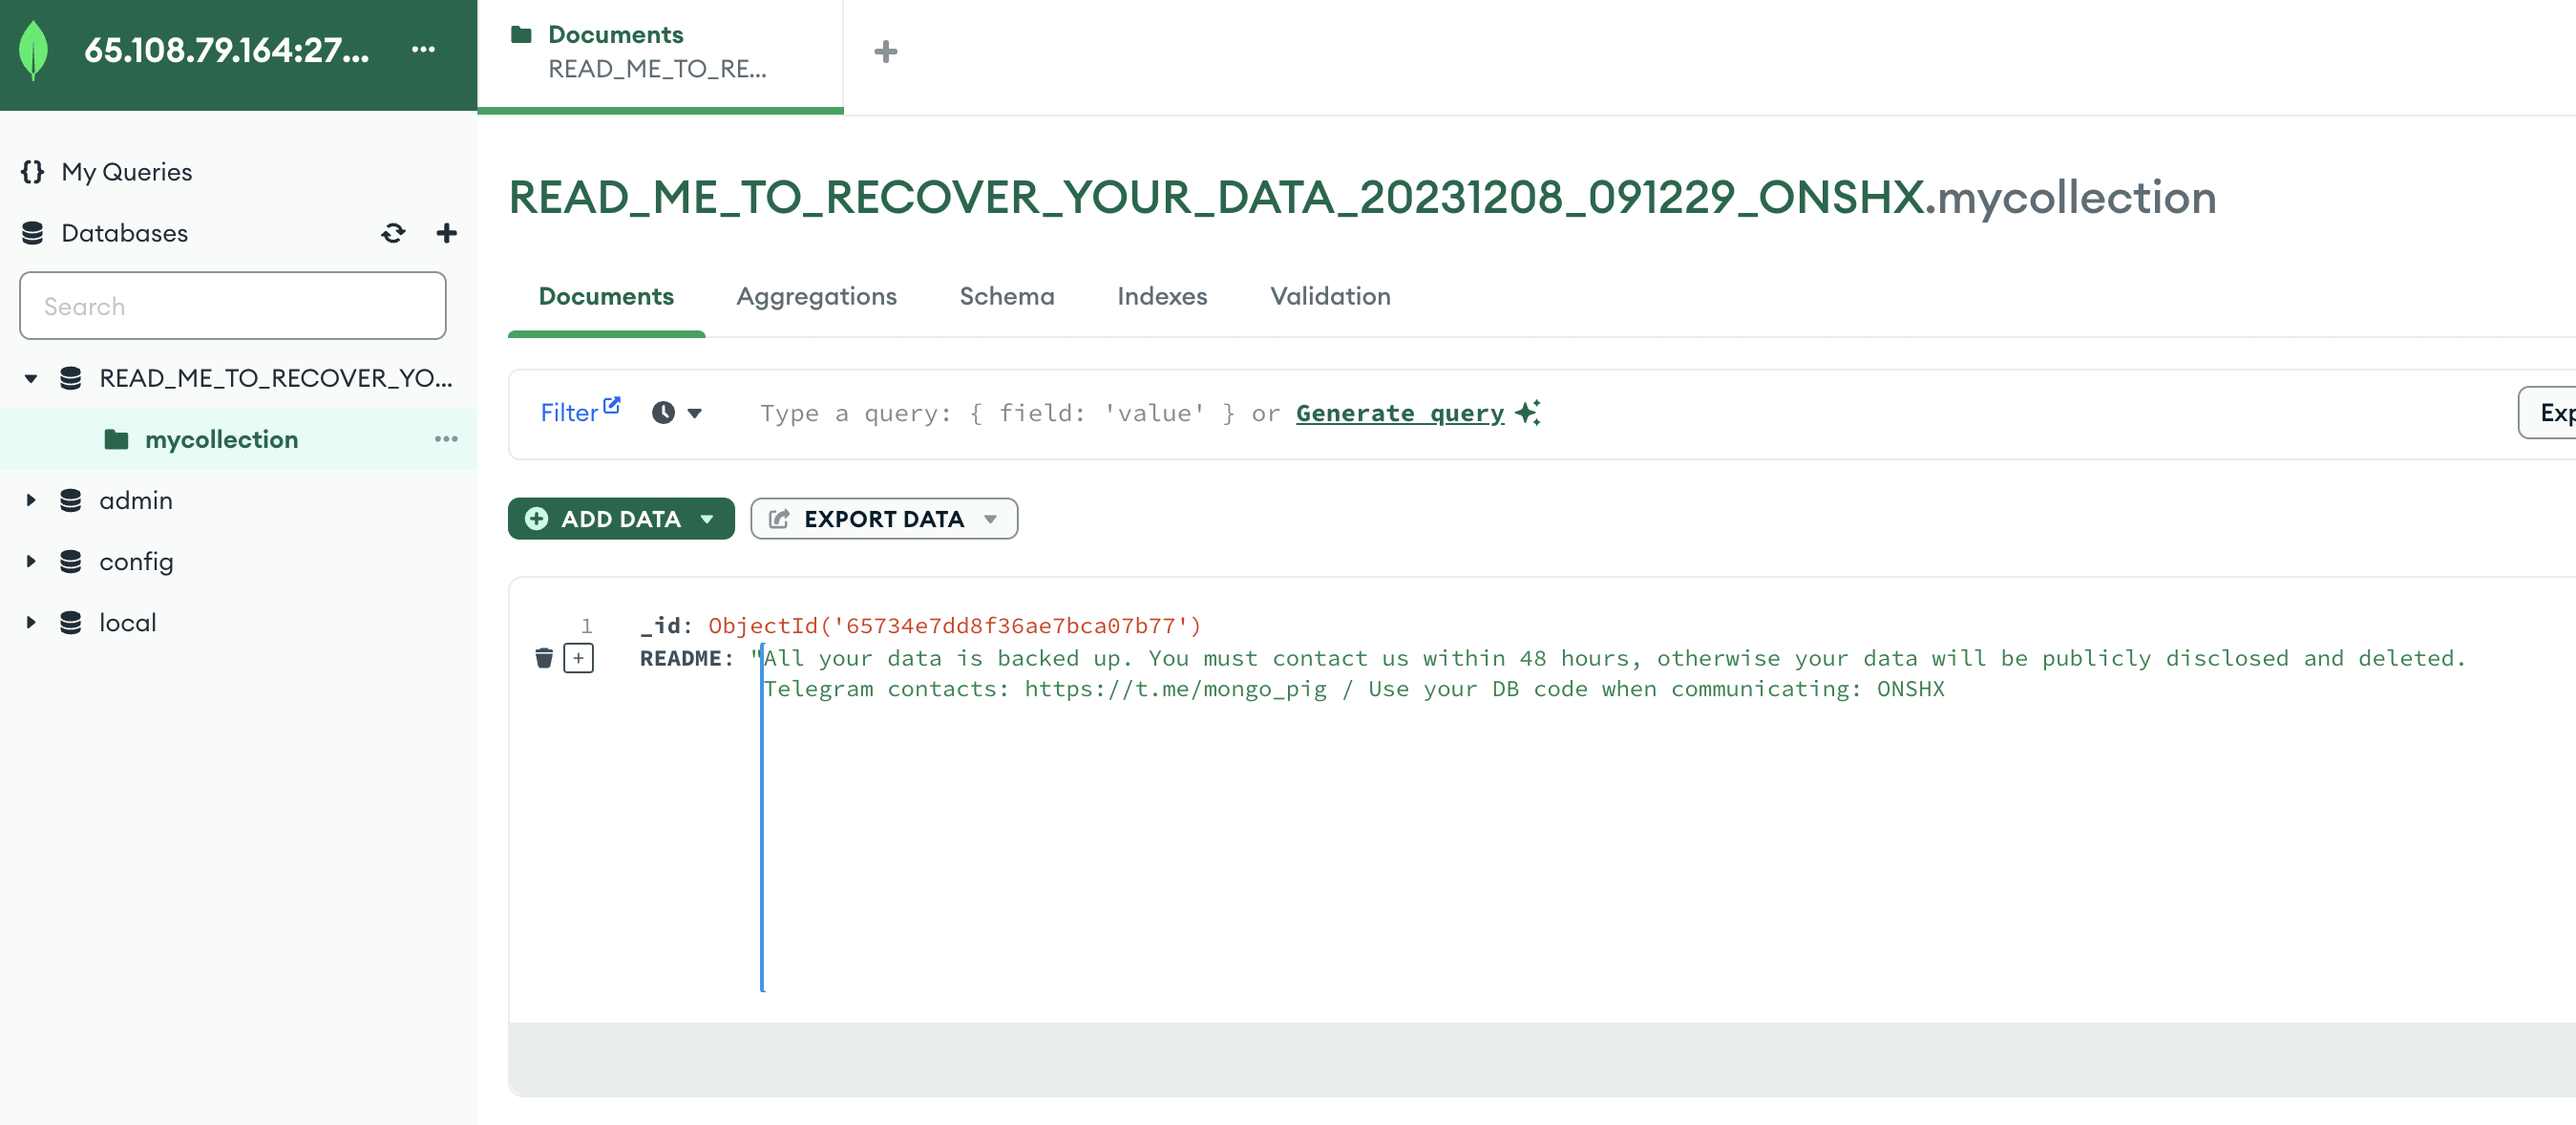
\includegraphics[width=0.9\linewidth]{doc/imgs/mongo-hack.png}
    \caption{Enter Caption}
    \label{fig:enter-label}
\end{figure}
\begin{figure}[H]
    \centering
    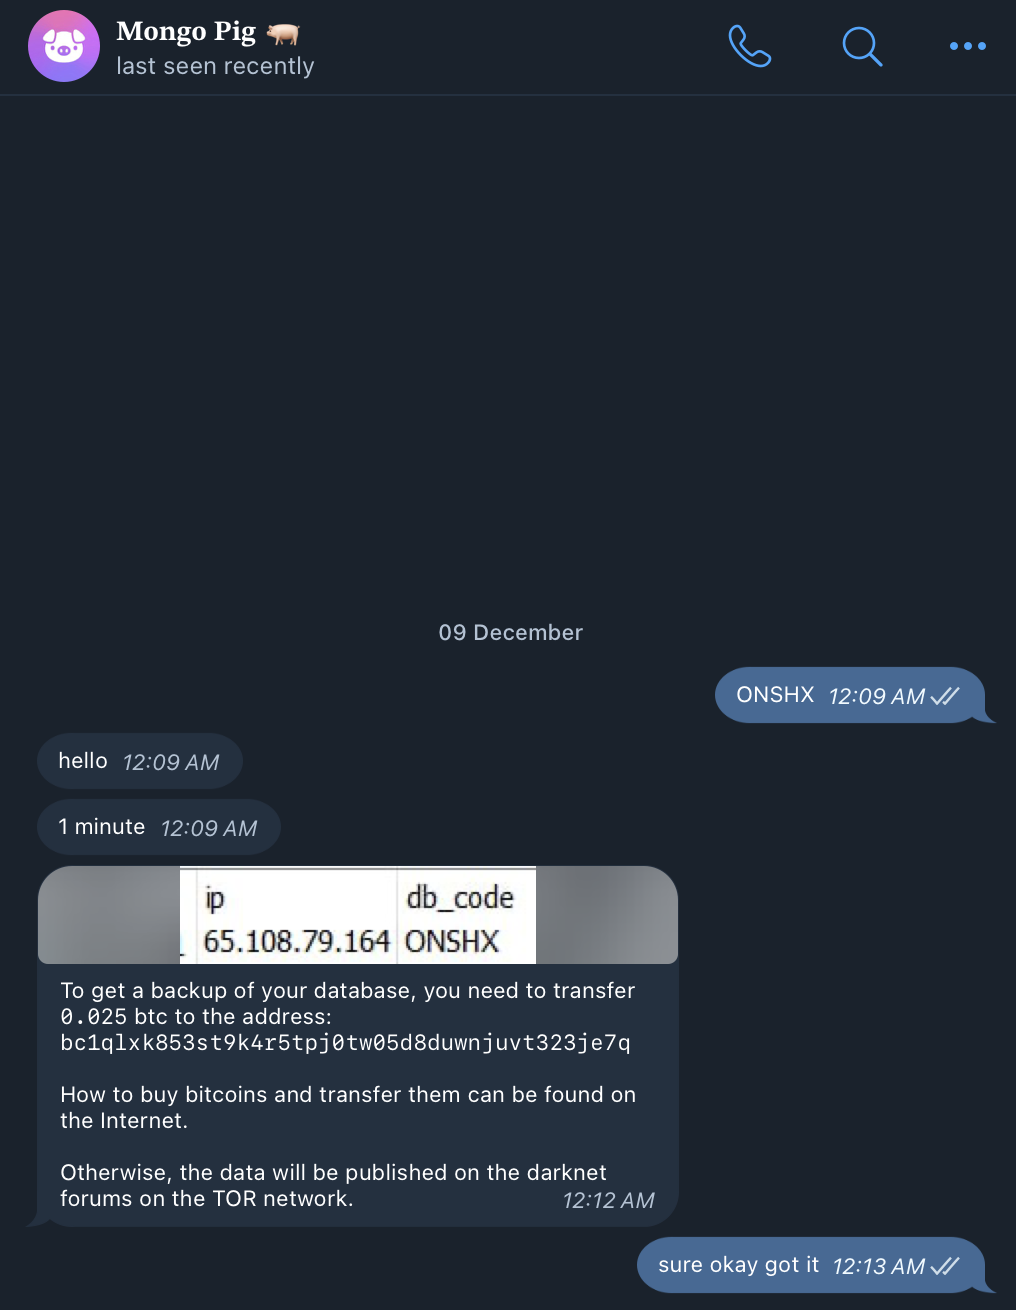
\includegraphics[width=0.5\linewidth]{doc/imgs/mongo-pig.png}
    \caption{Enter Caption}
    \label{fig:enter-label}
\end{figure}

\subsection{TLS/SSL}
MongoDB is one of several tools used in the system that have open connections to other services, together with RabbitMQ and the web servers. Each tool has its own security configurations and logging system to debug in case of errors. 
% Chương này có độ dài tối thiểu 5 trang, tối đa không giới hạn.\footnote{Trong trường hợp phần này dưới 5 trang thì sinh viên nên gộp vào phần kết luận, không tách ra một chương riêng rẽ nữa.} Sinh viên cần trình bày tất cả những nội dung đóng góp mà mình thấy tâm đắc nhất trong suốt quá trình làm ĐATN. Đó có thể là một loạt các vấn đề khó khăn mà sinh viên đã từng bước giải quyết được, là giải thuật cho một bài toán cụ thể, là giải pháp tổng quát cho một lớp bài toán, hoặc là mô hình/kiến trúc hữu hiệu nào đó được sinh viên thiết kế.

% Chương này \textbf{là cơ sở quan trọng} để các thầy cô đánh giá sinh viên. Vì vậy, sinh viên cần phát huy tính sáng tạo, khả năng phân tích, phản biện, lập luận, tổng quát hóa vấn đề và tập trung viết cho thật tốt.
% Mỗi giải pháp hoặc đóng góp của sinh viên cần được trình bày trong một mục độc lập bao gồm ba mục con: (i) dẫn dắt/giới thiệu về bài toán/vấn đề, (ii) giải pháp, và (iii) kết quả đạt được (nếu có).

% Sinh viên lưu ý \textbf{không trình bày lặp lại nội dung}. Những nội dung đã trình bày chi tiết trong các chương trước không được trình bày lại trong chương này. Vì vậy, với nội dung hay, mang tính đóng góp/giải pháp, sinh viên chỉ nên tóm lược/mô tả sơ bộ trong các chương trước, đồng thời tạo tham chiếu chéo tới đề mục tương ứng trong Chương 5 này. Chi tiết thông tin về đóng góp/giải pháp được trình bày trong mục đó.

% Ví dụ, trong Chương 4, sinh viên có thiết kế được kiến trúc đáng lưu ý gì đó, là sự kết hợp của các kiến trúc MVC, MVP, SOA, v.v. Khi đó, sinh viên sẽ chỉ mô tả ngắn gọn kiến trúc đó ở Chương 4, rồi thêm các câu có dạng: ``Chi tiết về kiến trúc này sẽ được trình bày trong phần 5.1". 


\end{document}